\documentclass{article}
\usepackage{amsmath}
\usepackage{amsthm}
\usepackage{amssymb}
\usepackage{enumerate}
\usepackage{pgfplots}

\makeatletter
\renewcommand{\abstractname}{Instructions}
\makeatother

\pgfplotsset{holdot/.style={color=blue,fill=white,only marks,mark=*}}

\title{MAT -- 112: Calculus I and Modeling\\
\large{Logarithm and Exponent Derivatives}}
\author{Instructor: Thomas R. Cameron}
\date{February 21, 2018}

\begin{document}
\maketitle

\begin{abstract}
Below is a list of trigonometric identities that you will need for today's class. 
\end{abstract}

\paragraph*{Trigonometric Identities.} Let $x,y$ be real numbers. Then
\begin{align*}
\sin^{2}x+\cos^{2}x &= 1 \\
\tan x &= \frac{\sin x}{\cos x} \\
\sin(x+y) &= \sin x\cos y + \sin y\cos x \\
\end{align*}

\paragraph*{An Important Lemma.}	Consider the graph below.
\begin{figure}
\centering
\begin{tikzpicture}[scale=0.75]
\begin{axis}[
	axis lines = left,
	legend pos = outer north east,
	xlabel = $x$,
	ylabel = $y$,
	ymin=-0.3, ymax=1,
]
\addplot[
	domain = -2*pi:2*pi,
	samples = 200,
	color = blue,
]
{sin(deg(x))/x};
\addlegendentry{$\frac{\sin x}{x}$}
\addplot [holdot] coordinates{(0,1)};
\end{axis}
\end{tikzpicture}
\end{figure}

\newpage

\paragraph*{Application.} A simple pendulum, see figure below, consists of a mass $m$ 
\begin{figure}[h]
\centering
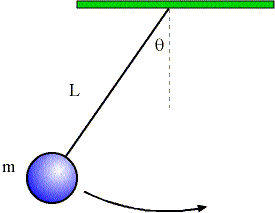
\includegraphics[scale=0.5]{../reviews/review1_fig1}
\end{figure}\\
hanging from a string of length $L$ from a fixed pivot point. When displaced to an initial angle $\theta_{0}$ and released, the pendulum will swing back and forth with periodic motion described by the equation
\[
\theta(t)=\theta_{0}\cos(\sqrt{\frac{g}{L}}t),
\]
where $g$ is the force of gravity and $t$ is the time elapsed since the mass was released. 
\begin{enumerate}
\item	Find an expression for $\theta^{'}(t)$.
\item	Evaluate $\theta^{'}(t)$ at the points $t$ where the displacement is maximized and zero. Interpret your results. 
\end{enumerate}

\end{document}